\newcommand{\gptpart}{5}
\newcommand{\gpttitle}{Graviton Pressure Theory}
\newcommand{\gptsubtitle}{Causality Restored: The Mechanics of Gravitational Force}
\newcommand{\gptdate}{November 2026}
% Shared preamble for the second edition of Graviton Pressure Theory.
% A part's own file sets \gptpart, \gpttitle, \gptsubtitle and \gptdate, then % Shared preamble for the second edition of Graviton Pressure Theory.
% A part's own file sets \gptpart, \gpttitle, \gptsubtitle and \gptdate, then % Shared preamble for the second edition of Graviton Pressure Theory.
% A part's own file sets \gptpart, \gpttitle, \gptsubtitle and \gptdate, then \input{../common/preamble}.
\documentclass[11pt,a4paper]{article}
\usepackage[T1]{fontenc}
\usepackage[utf8]{inputenc}
\usepackage{mathpazo}
\usepackage[scaled=0.92]{helvet}
\usepackage{amsmath,amssymb}
\usepackage[margin=2.5cm]{geometry}
\usepackage{microtype}
\usepackage{graphicx}
\usepackage{booktabs,array,tabularx}
\usepackage[font=small,labelfont=bf]{caption}
\usepackage{enumitem}
\usepackage[authoryear,round]{natbib}
\usepackage{titlesec}
\usepackage[titles]{tocloft}
\renewcommand{\cftsecfont}{\bfseries}\renewcommand{\cftsecpagefont}{\bfseries}
\renewcommand{\cftsecleader}{\hfill}\setlength{\cftsecnumwidth}{3.2em}
\usepackage{gpt-status}
\usepackage[hidelinks]{hyperref}
\setlength{\parskip}{4pt}
\setlength{\emergencystretch}{3em}
\setlength{\parindent}{0pt}
\setlist{itemsep=2pt,topsep=3pt}
\titleformat{\section}{\Large\bfseries}{\thesection}{1em}{}
\titleformat{\subsection}{\large\bfseries}{\thesubsection}{1em}{}
\renewcommand{\thesection}{\gptpart.\arabic{section}}
\renewcommand{\thetable}{\gptpart.\arabic{table}}
\renewcommand{\thefigure}{\gptpart.\arabic{figure}}
\renewcommand{\theequation}{\gptpart.\arabic{equation}}
\setcounter{tocdepth}{1}
\makeatletter\renewcommand{\@pnumwidth}{2.2em}\renewcommand{\@tocrmarg}{3em}
\makeatother
\bibliographystyle{plainnat}
\newcommand{\gptitle}{%
  \begin{titlepage}\centering
  \vspace*{3cm}
  {\Huge\bfseries Graviton Pressure Theory\par}\vspace{0.8cm}
  {\Large The Unified Framework\par}\vspace{0.2cm}
  {\large Individual Submission\par}\vspace{0.6cm}
  {\normalsize This document is part of a multi-part scientific framework\par}\vspace{2cm}
  {\normalsize Part \gptpart\ of 30\par}\vspace{0.8cm}
  {\huge\bfseries \gpttitle\par}\vspace{0.6cm}
  {\Large \gptsubtitle\par}\vspace{1.5cm}
  {\small\begin{minipage}{0.75\textwidth}\centering This submission is part of the broader Graviton Pressure Theory (GPT) project, a redefinition of gravitational interaction rooted in causal field dynamics and physical force transmission. Each document is designed to stand on its own; its full context emerges as part of the larger framework. For the complete series, see https://peopleoftheworld.net/graviton-pressure-theory/.\end{minipage}\par}
  \vfill
  {\large Author: Shareef Ali Rashada\par}\vspace{0.2cm}
  {\normalsize shareef@peopleoftheworld.net\par}\vspace{0.5cm}
  {\normalsize Second edition, \gptdate\par}
  \end{titlepage}
  \setcounter{page}{1}\tableofcontents\clearpage}
.
\documentclass[11pt,a4paper]{article}
\usepackage[T1]{fontenc}
\usepackage[utf8]{inputenc}
\usepackage{mathpazo}
\usepackage[scaled=0.92]{helvet}
\usepackage{amsmath,amssymb}
\usepackage[margin=2.5cm]{geometry}
\usepackage{microtype}
\usepackage{graphicx}
\usepackage{booktabs,array,tabularx}
\usepackage[font=small,labelfont=bf]{caption}
\usepackage{enumitem}
\usepackage[authoryear,round]{natbib}
\usepackage{titlesec}
\usepackage[titles]{tocloft}
\renewcommand{\cftsecfont}{\bfseries}\renewcommand{\cftsecpagefont}{\bfseries}
\renewcommand{\cftsecleader}{\hfill}\setlength{\cftsecnumwidth}{3.2em}
\usepackage{gpt-status}
\usepackage[hidelinks]{hyperref}
\setlength{\parskip}{4pt}
\setlength{\emergencystretch}{3em}
\setlength{\parindent}{0pt}
\setlist{itemsep=2pt,topsep=3pt}
\titleformat{\section}{\Large\bfseries}{\thesection}{1em}{}
\titleformat{\subsection}{\large\bfseries}{\thesubsection}{1em}{}
\renewcommand{\thesection}{\gptpart.\arabic{section}}
\renewcommand{\thetable}{\gptpart.\arabic{table}}
\renewcommand{\thefigure}{\gptpart.\arabic{figure}}
\renewcommand{\theequation}{\gptpart.\arabic{equation}}
\setcounter{tocdepth}{1}
\makeatletter\renewcommand{\@pnumwidth}{2.2em}\renewcommand{\@tocrmarg}{3em}
\makeatother
\bibliographystyle{plainnat}
\newcommand{\gptitle}{%
  \begin{titlepage}\centering
  \vspace*{3cm}
  {\Huge\bfseries Graviton Pressure Theory\par}\vspace{0.8cm}
  {\Large The Unified Framework\par}\vspace{0.2cm}
  {\large Individual Submission\par}\vspace{0.6cm}
  {\normalsize This document is part of a multi-part scientific framework\par}\vspace{2cm}
  {\normalsize Part \gptpart\ of 30\par}\vspace{0.8cm}
  {\huge\bfseries \gpttitle\par}\vspace{0.6cm}
  {\Large \gptsubtitle\par}\vspace{1.5cm}
  {\small\begin{minipage}{0.75\textwidth}\centering This submission is part of the broader Graviton Pressure Theory (GPT) project, a redefinition of gravitational interaction rooted in causal field dynamics and physical force transmission. Each document is designed to stand on its own; its full context emerges as part of the larger framework. For the complete series, see https://peopleoftheworld.net/graviton-pressure-theory/.\end{minipage}\par}
  \vfill
  {\large Author: Shareef Ali Rashada\par}\vspace{0.2cm}
  {\normalsize shareef@peopleoftheworld.net\par}\vspace{0.5cm}
  {\normalsize Second edition, \gptdate\par}
  \end{titlepage}
  \setcounter{page}{1}\tableofcontents\clearpage}
.
\documentclass[11pt,a4paper]{article}
\usepackage[T1]{fontenc}
\usepackage[utf8]{inputenc}
\usepackage{mathpazo}
\usepackage[scaled=0.92]{helvet}
\usepackage{amsmath,amssymb}
\usepackage[margin=2.5cm]{geometry}
\usepackage{microtype}
\usepackage{graphicx}
\usepackage{booktabs,array,tabularx}
\usepackage[font=small,labelfont=bf]{caption}
\usepackage{enumitem}
\usepackage[authoryear,round]{natbib}
\usepackage{titlesec}
\usepackage[titles]{tocloft}
\renewcommand{\cftsecfont}{\bfseries}\renewcommand{\cftsecpagefont}{\bfseries}
\renewcommand{\cftsecleader}{\hfill}\setlength{\cftsecnumwidth}{3.2em}
\usepackage{gpt-status}
\usepackage[hidelinks]{hyperref}
\setlength{\parskip}{4pt}
\setlength{\emergencystretch}{3em}
\setlength{\parindent}{0pt}
\setlist{itemsep=2pt,topsep=3pt}
\titleformat{\section}{\Large\bfseries}{\thesection}{1em}{}
\titleformat{\subsection}{\large\bfseries}{\thesubsection}{1em}{}
\renewcommand{\thesection}{\gptpart.\arabic{section}}
\renewcommand{\thetable}{\gptpart.\arabic{table}}
\renewcommand{\thefigure}{\gptpart.\arabic{figure}}
\renewcommand{\theequation}{\gptpart.\arabic{equation}}
\setcounter{tocdepth}{1}
\makeatletter\renewcommand{\@pnumwidth}{2.2em}\renewcommand{\@tocrmarg}{3em}
\makeatother
\bibliographystyle{plainnat}
\newcommand{\gptitle}{%
  \begin{titlepage}\centering
  \vspace*{3cm}
  {\Huge\bfseries Graviton Pressure Theory\par}\vspace{0.8cm}
  {\Large The Unified Framework\par}\vspace{0.2cm}
  {\large Individual Submission\par}\vspace{0.6cm}
  {\normalsize This document is part of a multi-part scientific framework\par}\vspace{2cm}
  {\normalsize Part \gptpart\ of 30\par}\vspace{0.8cm}
  {\huge\bfseries \gpttitle\par}\vspace{0.6cm}
  {\Large \gptsubtitle\par}\vspace{1.5cm}
  {\small\begin{minipage}{0.75\textwidth}\centering This submission is part of the broader Graviton Pressure Theory (GPT) project, a redefinition of gravitational interaction rooted in causal field dynamics and physical force transmission. Each document is designed to stand on its own; its full context emerges as part of the larger framework. For the complete series, see https://peopleoftheworld.net/graviton-pressure-theory/.\end{minipage}\par}
  \vfill
  {\large Author: Shareef Ali Rashada\par}\vspace{0.2cm}
  {\normalsize shareef@peopleoftheworld.net\par}\vspace{0.5cm}
  {\normalsize Second edition, \gptdate\par}
  \end{titlepage}
  \setcounter{page}{1}\tableofcontents\clearpage}

\graphicspath{{figs/}}
\begin{document}
\gptitle

\section*{About This Paper}
\addcontentsline{toc}{section}{About This Paper}

Every advance in physics begins not with an answer, but with a refusal to accept a placeholder. Parts 1 to 4 set out the refusal: gravity is described with great precision, and its cause is left unnamed. This paper sets out what Graviton Pressure Theory puts in its place, in one piece, so that the claims of Parts 6 to 13 can be read with the mechanism in hand.

It is written for that purpose. Each section gives one part of the mechanism: what it is, what touches what, what is exchanged, and what it is measured against. It does not derive everything; the derivations are in Parts 14 to 28, and each section says where. A table at the end shows which part of the mechanism each of Parts 6 to 13 relies on.

The whole of it is short enough to state at once. \hypm{Space is filled with a medium. Matter is a pattern of that medium, kept in being by taking it in; so the medium flows into every mass, and its pressure is lowered where it flows fastest. Every body in the flow is carried by it, and every clock and rod in it is slowed and squashed by the medium streaming through.} Everything else in this paper follows that statement into its consequences.

This is the second edition; what changed from the first is listed at the end. Claims are marked by their status, as the key shows.

\statuskey

\section{From Description to Mechanism}

\subsection{The test}

\argm{A description is not a mechanism.} A formula that gives the right number says what happens and how much. It does not say what makes it happen. Newton's law gives the force between two masses and names no carrier; Newton himself thought action at a distance through nothing an absurdity, and left the cause open.\fn{newton1687} General relativity gives the motion as geometry and names no exchange between matter and geometry (Part 8).\fn{rashadaPart8} Both are accurate. Neither answers the child who asks what holds her to the ground.

So every explanation in this framework, the mainstream's and GPT's alike, is held to one test: \argm{does it name what touches what, and what is exchanged?} A name is not an answer. ``Curvature'', ``potential energy'', ``pull'' and ``field'' are names; each says that something happens and stops before saying what does it (Parts 1 and 2).\fn{rashadaPart1}

\subsection{Four errors the test catches}

\begin{itemize}
\item \textbf{The Reduction Conflation} (Part 3).\fn{rashadaPart3} Two accounts that give the same numbers are taken to say the same thing about what exists. Matching numbers are not matching mechanisms: one solution of general relativity can be read as curved space or as a medium flowing in flat space, and the numbers cannot choose between them (Part 8).
\item \textbf{A force with no carrier} (Part 7).\fn{rashadaPart7} Push or pull, a force must say what touches what, where its energy comes from, and what pushes back. A pull is acceptable once its carrier is named, as with a rope. Gravity's pull has never had one.
\item \textbf{The Rest-and-Isolation Assumption} (Part 6).\fn{rashadaPart6} Physics usually begins with a body at rest, alone, in nothing. No real body is either. Every body is moving through several flows at once, and every action of a body happens in something.
\item \textbf{The idealisation taken for the event} (Part 28).\fn{rashadaPart28} An idealisation (a vacuum, a point mass, a frictionless plane) may approximate. It may not decide what exists. ``Empty space'' is the case: physics computes as if nothing were there, and then adds back what space contains as corrections, constants and new entities, so that nothing space does can enter as a cause.
\end{itemize}

\argm{Pressure is the language of physical contact.} It is what a hand feels holding a weight, what a wall returns, what a floor gives back. GPT proposes that gravity is spoken in the same language, and names the thing that speaks it.

\section{The Medium}

\subsection{Space is full}

\argm{Space is not empty, and the measurements say so.} The vacuum has a permittivity and a permeability, measured on the bench; together they set the speed of light, $c = 1/\sqrt{\mu_0\varepsilon_0}$, and the impedance every antenna is matched to, 376.73 ohms (Part 28). Space carries waves of gravity at the speed of light, with energy (Part 8). Empty of matter, it holds energy, about $5\times10^{-10}$ joules in every cubic metre.\fn{planck2018vi} It has a frame of rest, seen in the dipole of the background light, about 370 km/s.\fn{fixsen2009} In 1920 Einstein said that space without an ether is unthinkable.\fn{einstein1920}

\begin{hypbar}
\textbf{The medium.} Space is filled with a medium. Its constituent is what GPT calls the graviton: not the mainstream's hypothetical quantum of a gravitational wave, but the thing that everything else (matter, light, fields) is a pattern of (Part 15).\footnotemark{} The medium is not a gas of separate particles drifting through emptiness; it is the background in which all motion and all structure occur.
\begin{itemize}
\item \textbf{It has a pressure.} Gravitons in step with one another push each other apart, so the medium is self-repelling and presses on what is in it. Its undisturbed pressure is about $4.5\times10^{-10}$ pascals, from a density of about $10^{-26}$ kilograms in a cubic metre moving at $c$: $P_0 = \tfrac12\rho c^2$ (Part 24).
\item \textbf{Phase decides push.} Whether two parts of the medium push each other depends on their phase, the timing of their oscillation. In step, they push; out of step, they pass without pressing. The same rule, at the scale of atoms, gives contact and the bond (Parts 15 and 19).
\item \textbf{It carries waves.} Light is a transverse wave of the medium, and so is a gravitational wave; both travel at the speed the medium's stiffness and inertia allow, which is $c$ (Part 28).
\end{itemize}
\end{hypbar}
\footnotetext{\citealp{rashadaPart15}.}

\hypm{Without matter, the medium has one way of moving: its own oscillation, everywhere and in no direction, pressing equally from every side.} Once matter forms, it has a second: flow. Each particle takes the medium in, so the medium flows into it, and out again as counterflow. And \argm{because no mass forms alone, every new body forms inside flows already set up by the matter around it, and adds its own} (Part 18).\fn{rashadaPart18}

\section{Matter in the Medium}

\begin{hypbar}
\textbf{Matter is a pattern of the medium, kept in being by taking the medium in.} An electron or a proton is motion of the medium at the speed of light, closed on itself in a knot so that it goes nowhere (Part 17).\footnotemark{} Its mass is that confined motion: energy slowed down. A pattern of moving medium is not a fixed object; like a whirlpool or a flame, it keeps its shape while its material changes. So every particle of matter continuously takes in the medium, in step with the medium around it; gives up the in-step energy to its own circulation; and sends the medium on, out of step, as a counterflow that does not press.
\end{hypbar}
\footnotetext{\citealp{rashadaPart17}.}

\argm{This is what the first edition meant by mass resisting coherent compression.} The medium arriving in step is turned out of step by the matter it enters; the matter does not stop the flow, it converts it. Three consequences follow, and Parts 6 to 13 use all three.
\begin{itemize}
\item \hypm{The intake makes the inflow.} Matter takes in the medium from every side, so the medium around it flows inward, and the more matter, the more flow.
\item \hypm{The intake is set by energy, not by size or material.} Each turn of a particle's circulation takes in a fixed share, so the intake follows the particle's energy, binding energy included. That is why every material, measured, is carried alike (Part 17).
\item \hypm{Mass is one quantity.} The mass that resists a change of motion and the mass that is carried by the medium are the same confined motion; that is why they are equal (Part 11).\fn{rashadaPart11}
\end{itemize}

\section{The Inflow}

\subsection{Speed, acceleration and pressure}

\begin{figure}[t]\centering
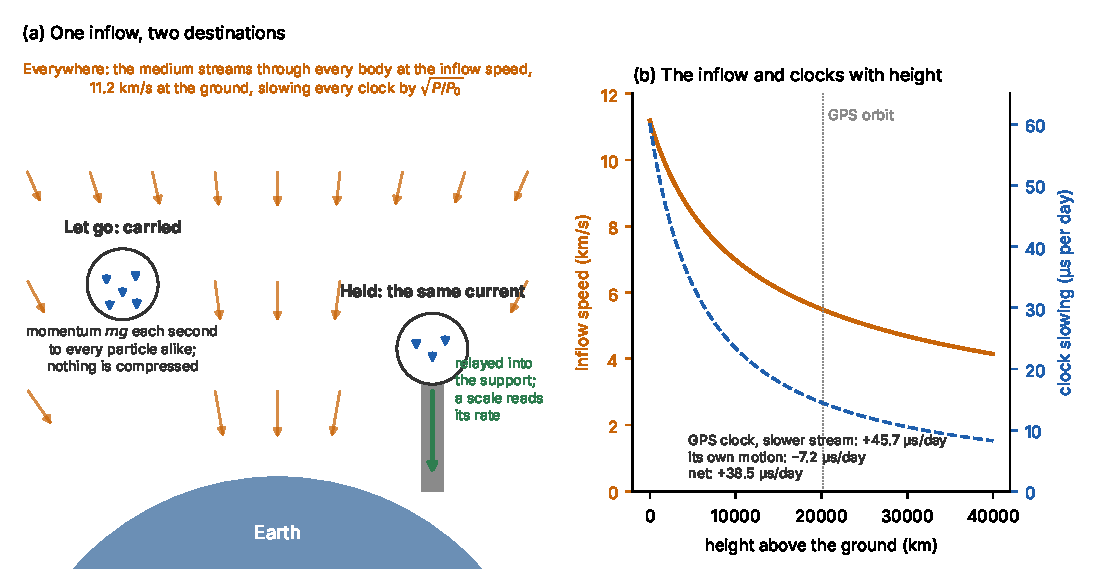
\includegraphics[width=\linewidth]{fig05-1-inflow.pdf}
\caption{The medium around the Earth. (a) The medium flows in from every side, faster lower down. A body that is let go is carried: momentum is delivered to each of its particles alike, so nothing inside it is compressed. A held body receives the same delivery and passes it into its support; that current is what a scale reads. (b) The inflow speed drops with height, from 11.2 km/s at the ground; a clock is slowed by the medium streaming past it, so a clock higher up runs faster. A GPS satellite's clock gains 45.7 microseconds a day from the slower stream and loses 7.2 from its own motion through the medium: 38.5 a day in all, as measured.}\label{fig:inflow}
\end{figure}

\begin{hypbar}
\textbf{The inflow.} Around a mass $M$, the medium flows inward at
\[ v = \sqrt{2GM/r}, \]
the Newtonian escape speed: 11.2 km/s at the Earth's surface, 618 km/s at the Sun's (Part 16).\footnotemark{} Flowing inward, the medium speeds up, and its own acceleration is
\[ a = GM/r^2, \]
the acceleration of Newton's law. Its pressure is lowered where it flows fastest, as a moving fluid's is:
\[ P/P_0 = 1 - v^2/c^2 = 1 - 2GM/rc^2. \]
At the Earth's surface the lowering is about one part in 700 million; at the Sun's, four parts in a million (Figure~\ref{fig:inflow}).
\end{hypbar}
\footnotetext{\citealp{rashadaPart16}.}

\argm{The inflow is calibrated, not fitted:} its speed is chosen so that its acceleration is Newton's, and from that one choice the pressure, the clock rates, the bending of light and the turning of Mercury's orbit all follow without further adjustment (Part 23).\fn{rashadaPart23} The same flow, written in the language of general relativity, is the Painlev\'e--Gullstrand form of the solution outside a mass, the ``river model'' of black holes.\fn{hamilton2008}

\subsection{The shadow, restated}

The first edition described a mass as casting a shadow in a flow of gravitons, with bodies pushed into the shadow. Two parts of that picture stand, and one does not.
\begin{itemize}
\item \argm{The region between two masses is a region of lowered pressure.} Each mass's inflow lowers the pressure around it, and between two masses both inflows act. In that sense ``shadow'' still describes it.
\item \hypm{Shading by absorption acts as well,} at the scale of the atom and possibly when bodies line up, as in eclipses. It is small: each particle takes only a tiny share of the medium passing through it, and measurements bound any shielding of gravity by matter far below what could carry weight (Part 15).
\item \argm{The force is carried by the flow, not by the shadow.} A body is not pushed into a shadow from behind; it is carried by the medium flowing around and through it. This is the first edition's river and stone, with the river flowing toward the mass, and the stone carried by it.
\end{itemize}

\section{Carried and Held}

This section is the mechanism Parts 6, 7 and 11 rely on most.

\subsection{Carried}

\begin{hypbar}
\textbf{A body let go is carried.} The medium streams through every body, and every particle of the body takes it in; so the medium delivers momentum to every particle at once, in proportion to its mass. A body of mass $m$ receives $mg$ of momentum each second, and shares the medium's acceleration $g$ (Part 7). It does not move with the medium; the medium still streams through it at close to 11.2 km/s. It shares the medium's acceleration, not its speed.
\end{hypbar}

\argm{This accounts for what is measured in free fall.}
\begin{itemize}
\item \textbf{Every body is carried alike.} Delivery is in proportion to mass, so the acceleration is the same for a feather and a hammer. Measured: titanium and platinum alike to about one part in $10^{15}$ (MICROSCOPE); the Earth and the Moon alike toward the Sun to about $10^{-13}$.\fn{touboul2022}\textsuperscript{,}\fn{williams2012}
\item \textbf{Nothing inside is compressed.} Delivery reaches every particle at once, so no part presses on another, and an accelerometer reads zero. A zero reading means uniform delivery, not no delivery: the acceleration is real, and is seen against any outside reference (Part 11).
\item \textbf{Free fall is not the absence of gravity; it is gravity unopposed.} It is permission: the medium carries, and nothing stops it.
\end{itemize}

\subsection{Held}

\begin{hypbar}
\textbf{A body held receives the same delivery and passes it on.} Holding is not a state in which nothing happens. The medium still streams through the held body and still delivers $mg$ of momentum every second; the body relays it, as compression, into its support, and the support into the ground (Part 6).\footnotemark{} The push appears only where the motion is stopped. That push is weight.
\end{hypbar}
\footnotetext{\citealp{rashadaPart6}.}

\begin{itemize}
\item \argm{One current, two destinations.} Held, the current passes into the support, and the scale reads its rate. Let go, it accumulates as motion, and an impact shows its total (Parts 6 and 11).
\item \argm{Holding is throughput, not consumption.} A table, an arch or a permanent magnet holds indefinitely with no input. Measured against the medium, momentum and energy flow through a held load (about 1.1 megawatts through 10 kilograms, at 11.2 km/s), and are passed on, not used up (Part 6). ``No work is done'' is true in the frame of the laboratory; it is not true in the medium's.
\item \hypm{Solidity is the boundary's answer.} Where two bodies meet, the counterflow from each, crowded at the contact, is brought back into step and presses. That pressure is the normal force: it resists compression, and creates and holds the boundary between the bodies. Its rate equals the momentum delivered, which is why every scale reading is a reading of the current (Parts 6 and 27).\fn{rashadaPart27} The first edition called this the compression barrier.
\end{itemize}

\subsection{Where the energy is}

\argm{A body carried toward the Earth gains energy, and in GPT the energy has an address.} \hypm{The medium pays it, from its pressure, converted into flow.} Lifting a body returns that energy to the medium's pressure; letting it go draws it back. ``Gravitational potential energy'' is the medium's pressure, located (Part 7). General relativity cannot say where gravitational energy is at any point (Part 8).

\subsection{Orbit}

\argm{An orbit is a body coasting sideways through a medium that is itself accelerating inward.} Nothing is paid to keep it going, and nothing inside it is compressed. The orbit closes because the inflow's acceleration weakens as the inverse square; it turns slowly, 43 arcseconds a century for Mercury, because \hypm{the medium's lowered pressure weakens the outward hold of the sideways motion} by the same factor that slows clocks (Part 26).\fn{rashadaPart26}

\section{Motion and Inertia}

The first edition described inertia as a corridor: a moving body takes in more of the medium ahead of it than behind, carving a path that favours continued motion, so that a change of motion costs the work of carving a new one. The second edition keeps the mechanism and states it in measured terms.

\begin{hypbar}
\textbf{Momentum is the carved path.} A body moving through the medium takes it in faster at its leading face than at its trailing face. That front-to-back imbalance is its momentum (Part 11). The exchange is wave-like: at speed $v$, the front rate is raised by a factor $k = \sqrt{(1+v/c)/(1-v/c)}$ and the back rate lowered by the same factor. Half their sum is $\gamma = 1/\sqrt{1-v^2/c^2}$, the energy factor; half their difference is $\gamma v/c$, the momentum factor. At six-tenths of the speed of light, $k = 2$, so the energy factor is 1.25 and the momentum factor 0.75.
\end{hypbar}

\begin{itemize}
\item \argm{Held steady, the path costs nothing.} The imbalance is kept without braking: orbits last, particles coast. This is what the first edition called the field's preference for continued motion.
\item \argm{Changing it costs.} A new speed or direction needs a new imbalance, and that is what a force pays for. Approaching $c$, the front rate grows without limit, so does the cost, and no body reaches the speed of light.
\item \hypm{The drag is inside.} The shared rate of the two faces is the body's rate at rest and runs its internal cycles; the excess carves the path. So a moving body's internal processes slow by $1/\gamma$: muons circulating at $\gamma \approx 29$ live 29 times longer.\fn{bailey1977}
\item \hypm{A gyroscope is a circulation.} Its spin is matter's circulation on a larger scale, set turning in the medium; reorienting it means reorienting that circulation, and the resistance is its angular momentum. The spinning Earth sets the medium around it turning, and a gyroscope's axis is carried by that swirl, measured by Gravity Probe B (Part 16).\fn{everitt2011}
\end{itemize}

\section{Clocks, Rods and Light}

This section is the mechanism Parts 8 and 10 rely on.

\begin{hypbar}
\textbf{A clock is slowed by the medium streaming past it.} A clock is a pattern of the medium whose cycles are carried by exchanges across it at $c$. Where the medium streams through it at speed $w$, the exchanges take longer, and every cycle slows by
\[ \sqrt{1 - w^2/c^2} = \sqrt{P/P_0}. \]
In the inflow, $w$ is the inflow speed, and the slowing is gravitational time dilation; for a moving clock, $w$ includes its own motion through the medium, and the slowing is motional. \textbf{They are one effect} (Parts 10 and 18).\footnotemark{}
\end{hypbar}
\footnotetext{\citealp{rashadaPart10}; \citealp{rashadaPart18}.}

\argm{The numbers follow with no fitted constant.} Two optical clocks a third of a metre apart in height run at measurably different rates; a gamma ray climbing 22.5 metres arrives shifted by 2.5 parts in $10^{15}$; and a GPS clock gains 38.5 microseconds a day, 45.7 from the slower stream at its height and $-7.2$ from its own motion (Figure~\ref{fig:inflow}).\fn{chou2010}\textsuperscript{,}\fn{pound1960}\textsuperscript{,}\fn{ashby2003}

\argm{Structure sets each clock's own rate; the medium sets a common slowing.} Temperature, stress and order change a clock's rate, and differ from clock to clock. The factor by which the medium's streaming slows that rate is the same for every kind of clock tested: nuclear, atomic, optical, and the decay of muons (Part 18).

\hypm{Rods are squashed along the flow by the same streaming.} A rod's bonds are kept up by exchanges across it; streaming lengthens the round trips more along the flow than across it, and the rod re-settles shorter along the flow by the same factor that slows the clock. One mechanism gives both factors, which is why they are equal. Space is flat; what general relativity calls stretched space is more of the squashed rods fitting in the same gap (Part 23).

\hypm{Light is refracted by the medium's lowered pressure.} Light is a wave of the medium and travels at $c$ through the medium where it is. Where the pressure is lowered, its index is raised: $n = P_0/P \approx 1 + 2GM/rc^2$. Passing the Sun's edge, light is bent 1.75 arcseconds and delayed, as measured; the standard account's own lensing calculations use the same index (Parts 8 and 10).\fn{schneider1992}\textsuperscript{,}\fn{bertotti2003}

\hypm{Redshift is the difference between clocks.} Light keeps the rhythm of its source; a source deep in the inflow is slowed, and the light carries that slower rhythm to where clocks run faster. The redshift is the same at every wavelength, as measured.\fn{okun2000}

\section{Many Bodies, Rotation and Time}

This section is the mechanism Parts 12 and 13 rely on, and the first edition's interference, corridors, memory and hysteresis restated.

\subsection{Many bodies}

\begin{itemize}
\item \hypm{Pressures combine; flows do not simply add.} Where two inflows meet, what combines is the medium's pressure, and every body is carried by the acceleration the combined pressure sets up (Part 7). This is the first edition's ``interference'': the medium is one, and the bodies in it share it.
\item \hypm{The forces are equal and opposite.} Each body receives momentum from the other's inflow in proportion to its own mass: $m \cdot GM/r^2$ and $M \cdot Gm/r^2$ (Part 7).
\item \argm{Tides are differences in carrying.} The Moon's inflow carries the near side of the Earth a little more than the centre, and the centre more than the far side: about $1.1\times10^{-6}$ m/s$^2$ at the surface. Large bodies amplify that small forcing into large signals: ocean basins into metres, soft layers into internal tides (Part 13).\fn{rashadaPart13}
\end{itemize}

\subsection{Rotation and the field in three dimensions}

\begin{hypbar}
\textbf{A field is the medium in motion around a mass: an inflow and a counterflow.} The inflow arrives from every side and carries bodies. The counterflow, the medium sent on out of step, carries the pattern of the body's spin and motion. A spinning body sets both turning, most strongly toward its equator and not at all along its axis, and the whole structure moves with the body through space (Part 16). Where the counterflow is brought back into step, at the distance where the inflow's acceleration has dropped to about $1.2\times10^{-10}$ m/s$^2$, the medium relaxes; this relaxation boundary is about 7,000 times the Earth's distance from the Sun for the Sun, and lies within the disc of a galaxy, where it gives the measured rotation of galaxies from their visible mass alone (Part 9).\footnotemark{}
\end{hypbar}
\footnotetext{\citealp{rashadaPart9}.}

\argm{The first edition's corridors are kept where they belong.} Inside matter, a corridor is a line of patterns held in step, along which the medium, load, heat and charge are passed (Part 21);\fn{rashadaPart21} a magnet is a corridor extended into the medium outside (Part 22).\fn{rashadaPart22} Between orbiting bodies, the counterflows meet in step at repeated conjunctions, and over long times systems are sorted into regular shells and resonances: the gaps in rings and in the asteroid belt, and the chains of planets in resonance (Parts 16 and 26).

\subsection{Time and the field}

\begin{itemize}
\item \argm{Changes in the field travel at the speed of light.} Gravitational waves and light from the same event arrived together, to about one part in $10^{15}$.\fn{abbott2017speed} The first edition's finite propagation delay stands, with its speed now measured.
\item \argm{The field keeps a record over time.} What the first edition called gravitational memory and hysteresis are measured where they are expected. Tides lag behind the Moon, because the oceans and the solid Earth take time to respond; the lag passes the Earth's spin to the Moon's orbit, and the Moon recedes 3.8 centimetres a year.\fn{dickey1994} Systems are sorted over long times into lasting resonances, and \hypm{a transition in a growing body may be biased by the configuration of the medium at that moment, and carry it as a record} (Part 13).
\end{itemize}

\section{What the Mechanism Must Pass}

\argm{GPT never argues against a measurement.} Every test result stands, and every part of the mechanism must pass it. Table~\ref{tab:pass} lists the outcome tests that constrain the whole mechanism, whatever its parts.

\begin{table}[t]\centering\small
\caption{The measurements every part of the mechanism must pass, and how it passes them.}
\begin{tabularx}{\linewidth}{@{}>{\raggedright}p{0.38\linewidth} X@{}}\toprule
\textbf{Measurement} & \textbf{How the mechanism passes}\\\midrule
Every material carried alike, to $10^{-15}$ \citep{touboul2022} & delivery in proportion to mass, set by energy\\
Gravity is not shielded by matter, to far below what weight needs & each particle takes a tiny share; the force is the flow (Part 15)\\
Gravitational waves at the speed of light, two transverse polarisations \citep{abbott2017speed} & transverse waves of the medium, at its wave speed\\
Every kind of clock slowed by the same factor \citep{chou2010,bailey1977} & the medium's streaming slows every cycle alike\\
The Earth's heat flow, about 47 terawatts & throughput is passed on, not deposited\\
Light bent 1.75 arcseconds; Mercury's orbit turned 43 arcseconds a century & the index $P_0/P$; the sideways hold weakened by $P/P_0$\\
Frame dragging, $37\pm7$ milliarcseconds a year \citep{everitt2011} & the medium's swirl\\\bottomrule
\end{tabularx}\label{tab:pass}\end{table}

\section{Reading Parts 6 to 13}

Table~\ref{tab:map} shows which part of the mechanism each of the next eight papers relies on, and where that part is derived in full.

\begin{table}[t]\centering\small
\caption{Parts 6 to 13: what each claims, the mechanism it relies on, and where the mechanism is set out here and derived in full.}
\begin{tabularx}{\linewidth}{@{}>{\raggedright}p{0.17\linewidth} >{\raggedright}p{0.33\linewidth} >{\raggedright}p{0.16\linewidth} X@{}}\toprule
\textbf{Part} & \textbf{Its central claim} & \textbf{Here} & \textbf{Derived}\\\midrule
6, Redefining Work & holding is throughput; the normal force is the current's signature & 5.5 & Parts 23, 27\\
7, The Illusion of Pull & every force names its carrier; free fall is permission, weight is push; energy located & 5.1, 5.5 & Parts 16, 23\\
8, Defining the Break & spacetime, if real, is a medium; the numbers cannot decide & 5.2, 5.4, 5.7 & Parts 14, 23\\
9, Existing Evidence & the medium already in the formulation; the relaxation boundary in galaxies & 5.2, 5.8 & Parts 16, 23\\
10, Practical Exploration & light refracted; clocks slowed by streaming; the tests & 5.7 & Parts 18, 23\\
11, Re-examining the Four & equivalence by uniform delivery; one current, two destinations & 5.3, 5.5 & Parts 17, 27\\
12, Materialist Epistemology & a description is not a mechanism & 5.1 & Parts 1, 2\\
13, The Moon and the Tides & tides as differences in carrying; amplification; the record & 5.8 & Parts 16, 26\\\bottomrule
\end{tabularx}\label{tab:map}\end{table}

\section*{Conclusion}
\addcontentsline{toc}{section}{Conclusion}

Graviton Pressure Theory does not ask the reader to believe in abstractions. It asks what touches what. Its answer is a medium that fills space; matter as a pattern of that medium, kept in being by taking it in; an inflow into every mass, with its pressure lowered where it flows fastest; and every body in it carried, every clock slowed and every rod squashed by the medium streaming through. Held, a body passes the medium's delivery into its support, and that is weight; let go, it is carried, and that is free fall. A moving body carves its path through the medium, and that is momentum. Light is refracted by the medium's lowered pressure, and that is lensing. A spinning body sets the medium turning, and that is frame dragging. Each gives the measured number, and each names its carrier.

Gravity is what happens when flow meets form. The first edition reclaimed it from the void that Newton and Einstein left unexamined. The second edition sets out what fills the void, and holds every part of it to the measurements.

\clearpage
\section*{Changes in the Second Edition}
\addcontentsline{toc}{section}{Changes in the Second Edition}

This list records what changed from the first edition and why. Changes to the argument alter what the paper claims or how it supports a claim; clarifications improve wording, sources or presentation and leave the argument as it was.

\subsection*{Changes to the argument}
\begin{itemize}
\item \textbf{The paper's role is stated.} It sets out the mechanism Parts 6 to 13 rely on, with a reading map, and points to Parts 14 to 28 for the derivations.
\item \textbf{Where the flow comes from.} The first edition described pre-existing currents of gravitons that mass interrupts. Kept and restated: before matter, the medium has only its own oscillation; once matter forms, it has flow as well, set up by matter taking the medium in; and every mass forms within flows already set by the matter around it, so for any particular body the flow does come first (Parts 16, 17 and 18).
\item \textbf{Mass.} ``Resistance to coherent compression'' is restated as matter converting the in-step medium it takes in (Part 17). The coherence resistance coefficient $\kappa_m$, the phase delay index $\delta_m$, and material-dependent gravitational response are withdrawn: every material is carried alike to $10^{-15}$. Where inside a structured body the delivery lands may depend on its order (Part 13).
\item \textbf{The force laws.} $\vec F_g = -\nabla\cdot\vec G$, $F = A(P_\text{in} - P_\text{out})$ and $\vec F = -\nabla(\rho_G v_G)$ are withdrawn: the force on a body does not scale with its area, and the first does not have the units of force. Replaced by the inflow, $v = \sqrt{2GM/r}$, and delivery in proportion to mass.
\item \textbf{The shadow.} The shadow as the cause of the force is replaced by the flow; the lowered pressure between masses and a small shading by absorption are kept, within the measured bounds.
\item \textbf{Free fall.} ``Uniform exposure to pressure on all sides'' and ``falling is the presence of pressure imbalance'' are replaced by carrying: momentum delivered to every particle in proportion to its mass. ``Pressure differential scales with resistance'' is replaced by delivery in proportion to mass.
\item \textbf{Weight and the ground.} ``Weight is resistance to graviton flow'' and the compression barrier are restated as the relayed current and the boundary's re-activated counterflow (Parts 6 and 27).
\item \textbf{Inertia and momentum.} The corridor and field-memory account of inertia is kept as the carved path, with its exact factors (front and back rates, $k$). The metaphors of the field's ``loyalty'', ``hospitality'' and ``intelligence'' are removed. Gyroscopic ``corridor shear'' is restated as the body's circulation and the medium's swirl.
\item \textbf{Withdrawn:} inertial weakening at the edge of coherence; field-structuring drives, inertial dampening and directional biasing for propulsion; the erasure of momentum by coherence engineering. No measurement supports them, and the bounds on shielding and on clock universality exclude the means.
\item \textbf{Corridors.} Corridors as channels holding planets in orbit, and as the explanation of flat rotation curves, are replaced by coasting orbits and the relaxation boundary (Parts 9 and 26). Corridors are kept inside matter and in magnets (Parts 21 and 22).
\item \textbf{Multi-body interference.} ``Superposition replaced by interference'' is restated as pressures combining; Lagrange points and resonances are restated as the long-time sorting of systems. Flow saturation in extreme systems is left to Part 25.
\item \textbf{Time.} Time dilation as coherence delay, with $\Delta t' = \Delta t(1 + \alpha\rho_G\delta_m)$ and material-dependent dilation, is withdrawn: every kind of clock is slowed alike. Replaced by the streaming medium, $\sqrt{P/P_0}$. Propagation delay is kept with its speed measured ($c$). Gravitational memory and hysteresis are restated as tidal lag, long-time sorting and the record of transitions.
\item \textbf{Lensing and redshift.} $\theta \propto \nabla\rho_G\,\ell$ is replaced by the index $n = P_0/P$. Redshift as ``oscillation drag'', with material dependence, is replaced by the difference between clocks.
\end{itemize}

\subsection*{Clarifications}
\begin{itemize}
\item The tone is changed: ``the time for metaphors has passed'', ``now, for the first time, it is explained'' and similar phrases are removed. ``Gravity as coherence'' is kept in the form ``gravity is what happens when flow meets form''.
\item The sections are reordered to follow the mechanism: the medium, matter, the inflow, carried and held, motion, clocks and light, many bodies.
\item One figure and two tables are added; sources are added for each measurement.
\end{itemize}

\bibliography{part05}
\end{document}
